% Options for packages loaded elsewhere
\PassOptionsToPackage{unicode}{hyperref}
\PassOptionsToPackage{hyphens}{url}
%
\documentclass[
]{article}
\usepackage{amsmath,amssymb}
\usepackage{lmodern}
\usepackage{iftex}
\ifPDFTeX
  \usepackage[T1]{fontenc}
  \usepackage[utf8]{inputenc}
  \usepackage{textcomp} % provide euro and other symbols
\else % if luatex or xetex
  \usepackage{unicode-math}
  \defaultfontfeatures{Scale=MatchLowercase}
  \defaultfontfeatures[\rmfamily]{Ligatures=TeX,Scale=1}
\fi
% Use upquote if available, for straight quotes in verbatim environments
\IfFileExists{upquote.sty}{\usepackage{upquote}}{}
\IfFileExists{microtype.sty}{% use microtype if available
  \usepackage[]{microtype}
  \UseMicrotypeSet[protrusion]{basicmath} % disable protrusion for tt fonts
}{}
\makeatletter
\@ifundefined{KOMAClassName}{% if non-KOMA class
  \IfFileExists{parskip.sty}{%
    \usepackage{parskip}
  }{% else
    \setlength{\parindent}{0pt}
    \setlength{\parskip}{6pt plus 2pt minus 1pt}}
}{% if KOMA class
  \KOMAoptions{parskip=half}}
\makeatother
\usepackage{xcolor}
\IfFileExists{xurl.sty}{\usepackage{xurl}}{} % add URL line breaks if available
\IfFileExists{bookmark.sty}{\usepackage{bookmark}}{\usepackage{hyperref}}
\hypersetup{
  pdftitle={Report},
  pdfauthor={Khalida Dushimova, Richard Efraim Langi, Madleen Piegsa, Greta Karathanos},
  hidelinks,
  pdfcreator={LaTeX via pandoc}}
\urlstyle{same} % disable monospaced font for URLs
\usepackage[margin=1in]{geometry}
\usepackage{graphicx}
\makeatletter
\def\maxwidth{\ifdim\Gin@nat@width>\linewidth\linewidth\else\Gin@nat@width\fi}
\def\maxheight{\ifdim\Gin@nat@height>\textheight\textheight\else\Gin@nat@height\fi}
\makeatother
% Scale images if necessary, so that they will not overflow the page
% margins by default, and it is still possible to overwrite the defaults
% using explicit options in \includegraphics[width, height, ...]{}
\setkeys{Gin}{width=\maxwidth,height=\maxheight,keepaspectratio}
% Set default figure placement to htbp
\makeatletter
\def\fps@figure{htbp}
\makeatother
\setlength{\emergencystretch}{3em} % prevent overfull lines
\providecommand{\tightlist}{%
  \setlength{\itemsep}{0pt}\setlength{\parskip}{0pt}}
\setcounter{secnumdepth}{-\maxdimen} % remove section numbering
\ifLuaTeX
  \usepackage{selnolig}  % disable illegal ligatures
\fi

\title{Report}
\author{Khalida Dushimova, Richard Efraim Langi, Madleen Piegsa, Greta
Karathanos}
\date{2022-07-12}

\begin{document}
\maketitle

\hypertarget{data-analysis-project-ss22}{%
\section{\texorpdfstring{\textbf{{DATA ANALYSIS PROJECT SS22
}}}{DATA ANALYSIS PROJECT SS22 }}\label{data-analysis-project-ss22}}

\hypertarget{proteome-wide-screen-for-rna-dependent-proteins}{%
\subsection{\texorpdfstring{\textbf{Proteome-wide Screen for
RNA-dependent
Proteins}}{Proteome-wide Screen for RNA-dependent Proteins}}\label{proteome-wide-screen-for-rna-dependent-proteins}}

\hypertarget{topic-03-team-04}{%
\subsection{\texorpdfstring{\textbf{Topic 03, Team
04}}{Topic 03, Team 04}}\label{topic-03-team-04}}

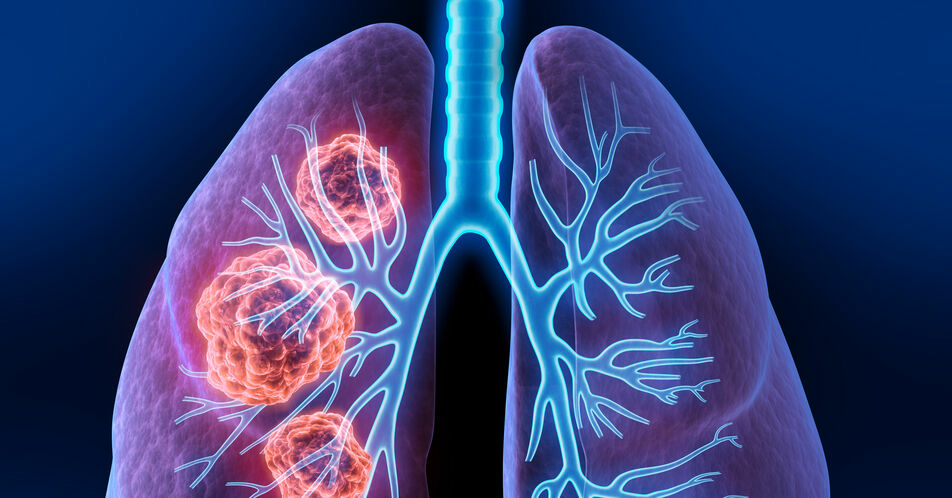
\includegraphics{../final/Lung_Cancer.png}

\hypertarget{deadline-18.07.2022}{%
\subsubsection{\texorpdfstring{\emph{Deadline:
18.07.2022}}{Deadline: 18.07.2022}}\label{deadline-18.07.2022}}

\begin{verbatim}
Supervisor: Dr. Maïwen Caudron-Herger

Tutor: Niklas Engel
\end{verbatim}

\hypertarget{molecular-biotechnology-4.fs}{%
\subsubsection{\texorpdfstring{\textbf{Molecular Biotechnology
4.FS}}{Molecular Biotechnology 4.FS}}\label{molecular-biotechnology-4.fs}}

\begin{verbatim}
Khalida Dushimova, Greta Karathanos, Richard Efraim Langi, Madleen Piegsa
\end{verbatim}

\hypertarget{introduction}{%
\section{1. Introduction}\label{introduction}}

RNA-dependent proteins are defined as RNA-dependent when their
interactome depends on RNA. This large group of proteins plays the key
roles in RNA processing and modification (Alternative splicing, RNA
editing and polyadenylation), export, mRNA localization and translation.
The malfunction of RNA-dependent proteins underlies the origin of many
diseases from muscular atrophies and neurological disorders to cancer.
Therefore, it is necessary to increase the number of recognized
RNA-dependent proteins and the understanding of their molecular
mechanisms. Since identifying molecular mechanisms is one of the biggest
challenges in (nc)RNA (-\textgreater{} non-coding), research
M.Caudron-Herger et al.~created R-Deep to detect RNA-dependent proteins
automatically. In general, R-Deep is a proteome-wide, unbiased, and
enrichment-free screen based on density gradient ultracentrifugation
(Caudron-Herger et al., 2019). Performing R-Deep, lysates with a
previous RNase treatment (RNase group) and without a previous RNase
treatment (Ctrl group) were separated by their density. Each fraction
was analyzed by mass spectrometry or western blot according to its
protein amount (Caudron-Herger et al., 2020). Detected RNA-dependent
proteins can bind directly to the RNA (RBP) or bind to RBPs.

\hypertarget{materials-and-methods}{%
\section{2. Materials and Methods}\label{materials-and-methods}}

\hypertarget{rdeep}{%
\subsection{2.1 RDeep}\label{rdeep}}

R-DeeP is a proteome-wide, unbiased and enrichment-free screen. The
principle of R-DeeP is based on cellular lysate fractionation by density
gradient ultracentrifugation. (Referenz) The outcome is analyzed by
proteome-wide mass spectometry or individual western blotting. In
general, R-DeeP is used to determine RNA-dependent proteins, that
interact directly or indirectly with RNA. Lysates with (RNase group) and
without (Ctrl group) RNase treatment are compared. By that differences
in molecular weight, hence and the size of the complexes are
determined.RBPs are expected to split after RNase treatment and migrate
to different fractions in a sucrose density gradient.

\hypertarget{dataset-exploration}{%
\subsection{2.2 Dataset exploration}\label{dataset-exploration}}

Our given dataset consists of mass-spectrometry data from
non-synchronized A549 cells which are human lung carcinoma cells of a
caucasian male. In general, the data show the protein amount of each of
our 3680 human proteins per fraction. The RDeep screen has been repeated
three times so it comprises three replicates for each sample. All in
all, we got 3680 rows with one human protein per row and 150 columns for
our Ctrl and RNase group for 25 fractions and three replicates each.

\hypertarget{first-normalization-fractionwise}{%
\subsection{2.3 First Normalization
(fractionwise)}\label{first-normalization-fractionwise}}

The total amount of protein of every replicate should be similar. In our
given dataset this was not the case. Normalization is the process to
account for the bias and make samples more comparable. The aim was to
change the values of columns to a common scale without distorting
differences in the range of values and by this reduced the variation
between our three technical replicates. Therefore, for our first
normalization, we compute the sums fractionwise and find the two closest
sums. We then define normalization factors for the replicates. The
quotients of the mean sums and sums of replicates are the normalization
factors.

\hypertarget{second-normalization-anti-outlier-function}{%
\subsection{2.4 Second Normalization (anti-outlier
function)}\label{second-normalization-anti-outlier-function}}

For our second normalization, we defined the mean out of the two most
similar replicates and by this wrote our own function to exclude
outliers. The outliers were found, removed, and replaced by the mean of
the other two most similar replicates.

\hypertarget{peaks-identification}{%
\subsection{2.5 Peaks identification}\label{peaks-identification}}

Peaks We expect RNA-dependent proteins to migrate to different positions
in the RNase-treated sample compared to the Ctrl sample. As a next step,
we identify the maxima in both samples to characterize a protein as RNA
dependent or RNA independent. We detected the local and the global
maxima to draw all the biological information we could get from our
given values. Our theoretical maximum is a point x whose neighboring
values have to be smaller {[}1{]}.

The method is based on checking the neighbors of each fraction. For the
first fraction, only the right neighbor will be compared because there
is no left neighbor. For the second to twenty-fourth fraction, both left
and right neighbours will be compared. For the last fraction, only the
left neighbour will be compared since the right neighbour doesn't exist.
If the checked fraction has higher values than the neighbor(s), then the
fraction is a maximum. If the the checked fraction have lower values
than the neighbour(s), then the fraction is not a maxima and will be
zero-ed in our code.

\hypertarget{criteria-for-rna-dependency}{%
\subsection{2.6 Criteria for RNA
dependency}\label{criteria-for-rna-dependency}}

\hypertarget{t-test-of-absolute-maxima}{%
\subsubsection{2.6.1 T-Test of absolute
maxima}\label{t-test-of-absolute-maxima}}

T Test is a statistical test under the null hypothesis and can be used
to determine the significance of the data. For our data, a two-sided
unpaired T-Test is performed with Bonferroni correction. The Bonferroni
correction is a method to adjust the significance level α to avoid a
type I error (rejecting the null hypothesis when you should not) when
performing multiple statistical tests. The formula for a
Bonferroni-correction is as follows: \(α_{new} = α_{originial} / n\).
T-Test allows us to determine if the global maxima of each of the
proteins (all replicates) between the Ctrl and RNase group have a
significant difference. We declare a significant difference between both
groups as RNA-dependent. It will be our first criterion for RNA
dependency.

\hypertarget{k-means-clustering-y-shift-and-x-shift-detection}{%
\subsubsection{2.6.2 K-Means Clustering (Y-shift and X-shift
detection):}\label{k-means-clustering-y-shift-and-x-shift-detection}}

K-Means Clustering is an unsupervised non-linear algorithm that clusters
data based on similarity. It aims is to partition the observations into
a previously defined number of clusters. We define this number by
performing the elbow method. Through K-Means Clustering and comparing
our t-test results, we define selection criteria (Y-shift and X-shift)
to determine RNA-dependent proteins. Y-shift is the difference in
protein amount between the global maxima of the Ctrl and RNase group.
X-shift is the difference of locations of global maxima (fraction)
between the global maxima of the Ctrl and RNase group.

If the X- and Y-shift have positive values (left and down shift), we
define the protein as RNA dependent. If the X- and Y-shift have negative
values or are close to zero (right and up shift), we define the protein
as RNA independent. These shifts will be our second criteria for RNA
dependency. We also combined our X- and Y-shifts in a data frame and
used the elbow method to determine the optimal number of clusters.

\hypertarget{t-test-of-local-maxima}{%
\subsubsection{2.6.3 T-Test of local
maxima:}\label{t-test-of-local-maxima}}

To find more RNA dependent proteins, we will include a 3rd criteria to
classify the protein as RNA dependent. The 3rd criterion is the result
of the t-test of local maxima. The same T Test principle from global
maxima is used.

\hypertarget{comparison-with-other-databanks}{%
\subsection{2.7 Comparison with other
databanks:}\label{comparison-with-other-databanks}}

To calculate the true positive and true negative rate and see how good
our criteria find the RNA dependent proteins we compare our findings
with mammalian RNA-binding protein resources
(\url{https://r-deep.dkfz.de})

\hypertarget{linear-regression}{%
\subsection{2.8 Linear regression:}\label{linear-regression}}

Finally, we perform a linear regression. This model can generally be
used to model the relationship between a dependent variable (regressand)
and one or more explanatory variables (predictors). The relationship is
represented by a linear function. We can see from the model to what
extent the dependent variable can be explained by the other variables.
Our regression model predicts the Y-Shift values with the information
from correlation between Ctrl and RNase.

\hypertarget{working-with-complementary-data}{%
\subsection{2.9 Working with complementary
data:}\label{working-with-complementary-data}}

We used an additional data bank from our tutor, Niklas Engel for our
second linear regression. The other one is from RDeep website and is
used to compare our results with it.

\hypertarget{results}{%
\section{3. Results}\label{results}}

\hypertarget{data-reorganization}{%
\subsection{3.1 Data Reorganization}\label{data-reorganization}}

The raw data was split into two data frames, one for Ctrl group
\textbf{Ctrl} and one for RNase \textbf{RNase} group. Each group
consists of 25 rows representing the fractions and 11040 columns
representing the 3680 proteins including the 3 Reps.

\hypertarget{data-evaluation}{%
\subsection{3.2 Data Evaluation}\label{data-evaluation}}

For further analysis of the replicates, we summed up the total protein
amount of all genes per replicate and plotted them side by side in a bar
chart. The total protein amount between each Reps of Ctrl and RNase
samples is very variable.

\hypertarget{first-normalization}{%
\subsection{3.3 First Normalization}\label{first-normalization}}

The results of our first normalization can be found in 2 data frames,
\textbf{Norm\_Ctrl} for Ctrl group and \textbf{Norm\_RNase} for RNase
group, each with 11040 rows representing the proteins with 3 Reps and 25
columns for the fractions. To check the results of our normalization, a
bar chart of total protein amount on the y-axis and each Rep of Ctrl and
RNase was created. The plot before normalization can be seen in {[}2{]}.

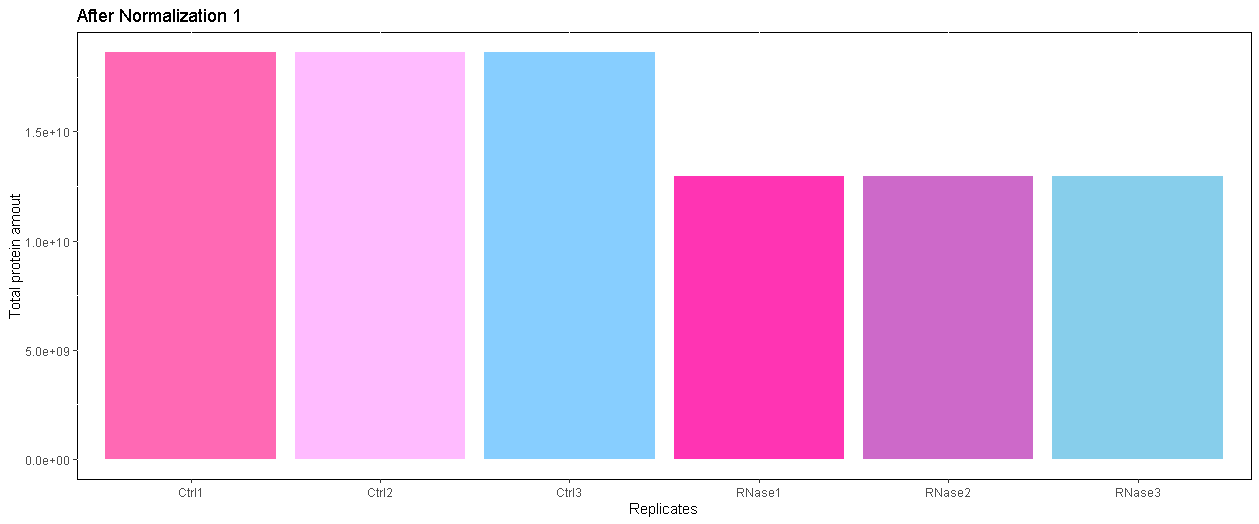
\includegraphics{../results/png/After_Norm_1.png} The bar chart revealed
that the three replicates of Ctrl and RNase have the same total amount.
The chart also showed that although the protein amount of all three
replicates of Ctrl and RNase is equal and there is a difference between
the total amount of Ctrl and RNase.

\hypertarget{second-normalization}{%
\subsection{3.4 Second Normalization}\label{second-normalization}}

The results of our second normalization from our
\textbf{df\_combi\_function} can be found in 2 data frames,
\textbf{tCtrl\_combi\_df} for Ctrl group and \textbf{tRNase\_combi\_df}
for RNase group, each with 11040 columns representing the proteins with
3 Reps and 25 rows for the fractions. To check the results of our
normalization, 3 graphs of 3 reps of a Protein
\textbf{MICA\_Human\_Ctrl} before and after normalization with the
fractions on x-axis and the protein amount on y-axis were produced. The
plot of before normalization can be seen in {[}3{]}.

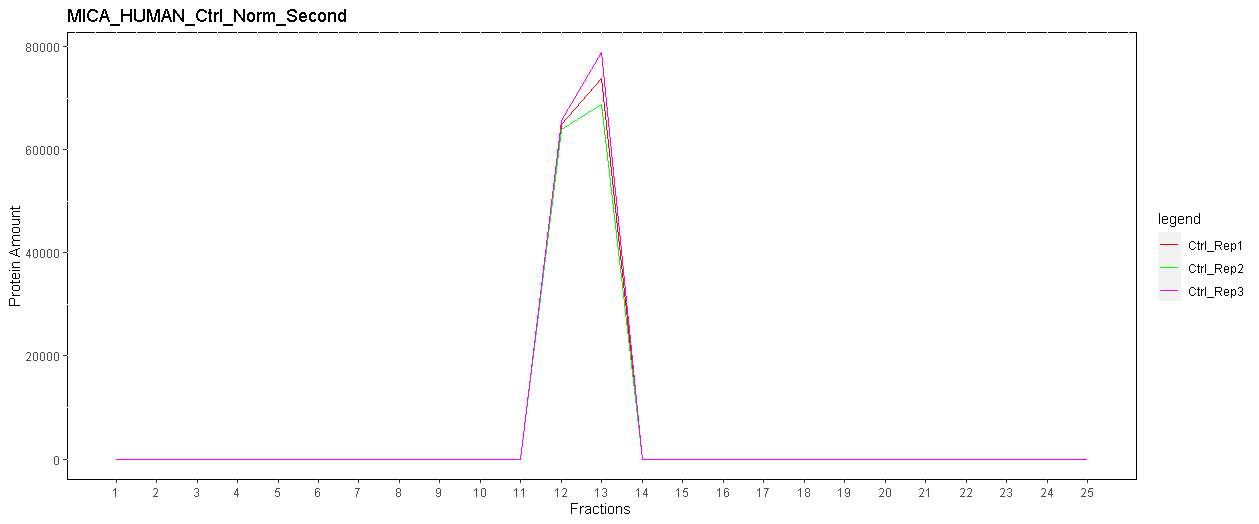
\includegraphics{../results/png/After_Norm_2.png} The 3 graphs of
normalized replicates revealed that the replicates have a similar amount
of protein and there are no more significant outliers left.

\hypertarget{peaks-identification-1}{%
\subsection{3.5 Peaks Identification:}\label{peaks-identification-1}}

Using our self-written \textbf{maximafunction}, 9 data frames were
received and each of them had a different threshold.
\textbf{maxima\_Ctrl\_i} is the result for the Ctrl group and
\textbf{maxima\_RNase\_i} for the RNase group, where \textbf{i}
represents the percentage of global maxima (threshold). \textbf{i} has
values between 0.1 - 0.9. The data frames consisted of 11040 columns
representing proteins including reps and 25 columns for fractions. The
values of protein amount of global (absolute) and local maxima were
presented whereas no maxima are zero-ed.~Our self-written
\textbf{maxnum\_plot\_col} produced a plot, which plotted a random
protein with all thresholds on the x-axis and the number of maxima on
the y-axis. An example plot can be seen in {[}4{]}.

\hypertarget{criteria-for-rna-dependency-1}{%
\subsection{3.6 Criteria for RNA
dependency}\label{criteria-for-rna-dependency-1}}

\hypertarget{t-test-of-global-and-local-maxima}{%
\subsubsection{3.6.1 T-Test of Global and Local
maxima:}\label{t-test-of-global-and-local-maxima}}

A data frame \textbf{test} with 3680 rows and one column was produced
after performing a t-test of global maxima between Ctrl and RNase group.
The rows represented the names of the proteins and were alphabetically
ordered. The column represented the RNA dependency with two kinds of
results, TRUE or FALSE.

For the t-test of local maxima, the results were presented in a data
frame \textbf{test\_0.4} that consists of 3680 rows and 1 column. The
name of the proteins was shown in the rows and the only column explained
the RNA dependency. Three outcomes were generated, TRUE, FALSE or NA.

\hypertarget{k-means-clustering}{%
\subsubsection{3.6.2 K-Means Clustering}\label{k-means-clustering}}

To find the optimal number of clusters, a plot of elbow method was used,
where the x-axis represented the number of clusters and the y-axis the
total within clusters sum of squares. The elbow method revealed a hard
kink for three clusters.

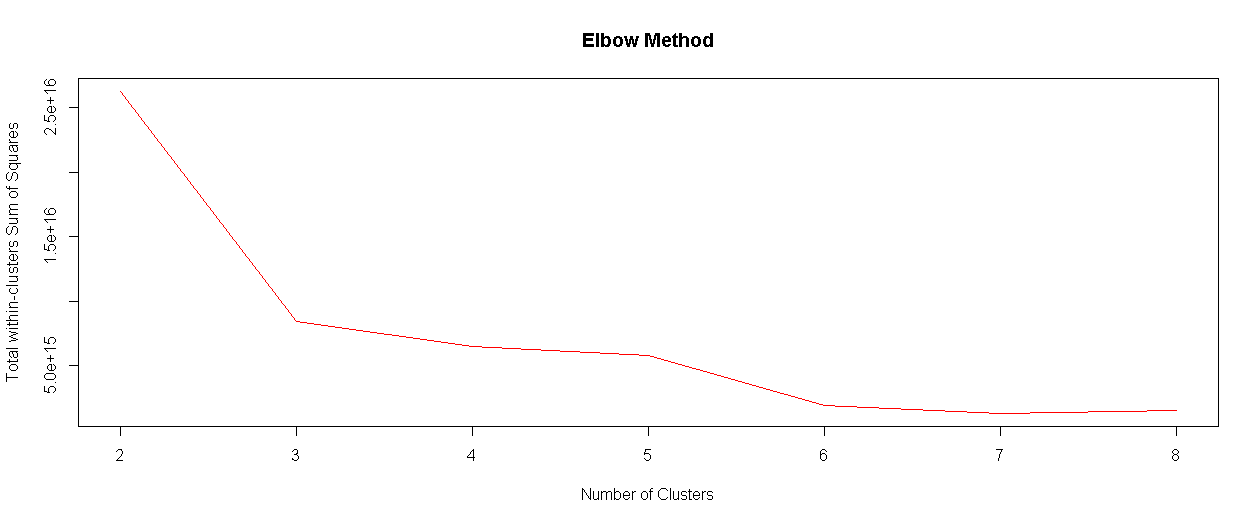
\includegraphics{../results/png/Elbow.png}

The result of k means clustering was shown in \textbf{km}. The values of
our within-cluster sum of squares of our 3 clusters were
2.275488e\textsuperscript{15}, 2.637920e\textsuperscript{15} and
3.487322e\textsuperscript{15}. Then, a plot of the y-shift on the y-axis
and x-shift on the x-axis was created to better visualize the cluster.
The second cluster had the most data points, then the first cluster and
lastly the third cluster with interestingly only 4 data points. What is
noticeable is that the second cluster has mostly positive x and y shift
values.

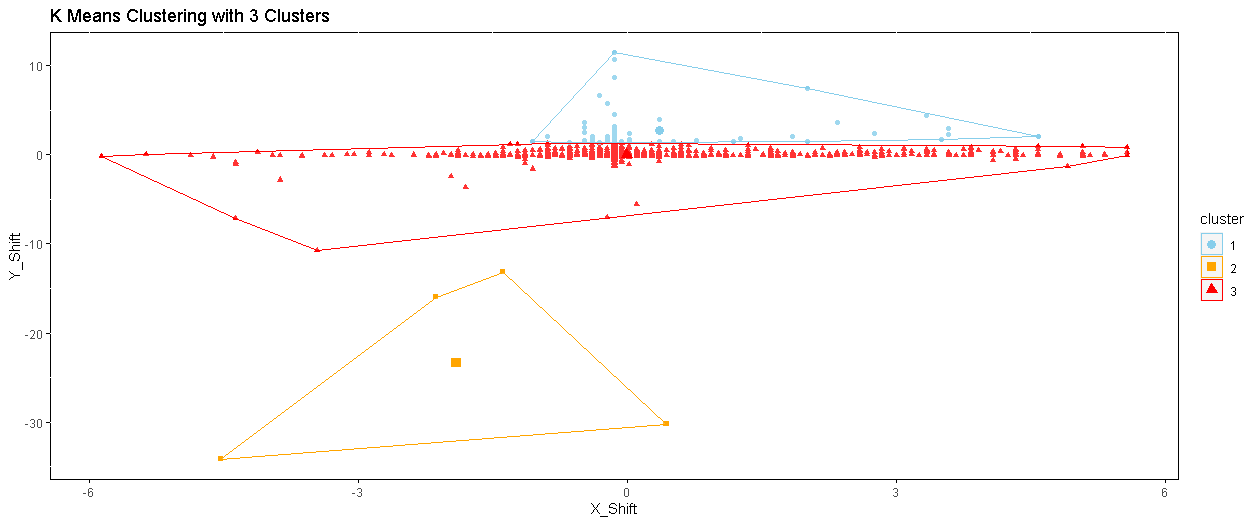
\includegraphics{../results/png/K_Means.png}

\hypertarget{comparison-with-data-bank-with-two-criteria}{%
\subsubsection{3.6.3 Comparison with Data Bank with two
Criteria}\label{comparison-with-data-bank-with-two-criteria}}

The results of the RNA dependent proteins (2 Criteria) were presented in
2 data frames. 305 proteins \textbf{Ctrl\_Dependent\_Abmax\_1} were
identified when one of the two criteria was fulfilled and 63 proteins
\textbf{Ctrl\_Dependent\_Abmax\_2} when both criteria were fulfilled.

To check how many RNA dependent proteins were ``correctly'' identified,
our results were compared with a data bank
\textbf{table\_RBP\_lists.csv} from RDeep website. Out of 63 identified
RNA-dependent proteins that fulfill both criteria, 58 had a match with
the comparable data bank when both criteria are fulfilled
(\textbf{RDeep\_2}) and for either criteria fulfilled out of 305
identified proteins 233 have matches (\textbf{RDeep\_1}). Unfortunately,
our applied criteria could not identify 2017 RNA dependent proteins
(\textbf{Not\_identified\_RDeep\_1}).

\hypertarget{comparison-with-data-bank-with-three-criteria}{%
\subsubsection{3.6.4 Comparison with Data Bank with three
Criteria}\label{comparison-with-data-bank-with-three-criteria}}

The results of the RNA dependent proteins (3 Criteria) were presented in
a data frame \textbf{dependent\_3} where 472 proteins were classified as
RNA-dependent. Out of 472 identified RNA-dependent proteins that fulfill
either criteria, 364 had a match (\textbf{RDeep\_3}). Unfortunately our
applied criteria could not identify 1886 RNA dependent
(\textbf{Not\_identified\_RDeep\_3}).

\hypertarget{linear-regression-1}{%
\subsection{3.7 Linear Regression}\label{linear-regression-1}}

The first linear regression was performed between the correlation of
Ctrl and RNase absolute maxima for the x-axis and y-shift for y-axis.
The linear equation from the regression was \(y = 1690907x - 1184175\).
The p-value for the predictor variable y was 7.98e\textsuperscript{-06}
and for x is 5.96e\textsuperscript{-09}. The p-value of our model was
5.962e\textsuperscript{-09} (\textbf{lm}). The linear regression can be
seen in {[}5{]}. The QQ plot of the theoretical and sample residues
aligned with the QQ line except when the theoretical quantiles were
below -2.5 and above 2.5. The residuals were also plotted in a histogram
{[}6{]}.

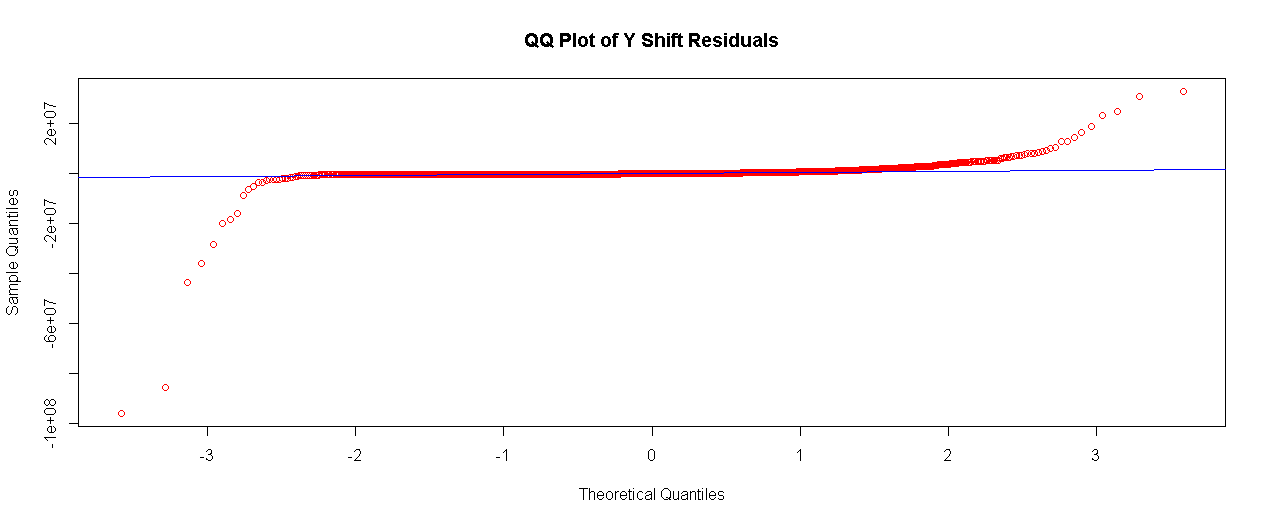
\includegraphics{../results/png/QQ_Y.png}

The last plot was a plot with actual value on x-axis, predicted value on
y-axis and a linear line with intercept 0 and slope 1. The data points
gather mostly in the place where the predicted and actual values are
above 0. Below 0 there were only a few points that are near the linear
line. Nonetheless, some points are very far from the linear line.

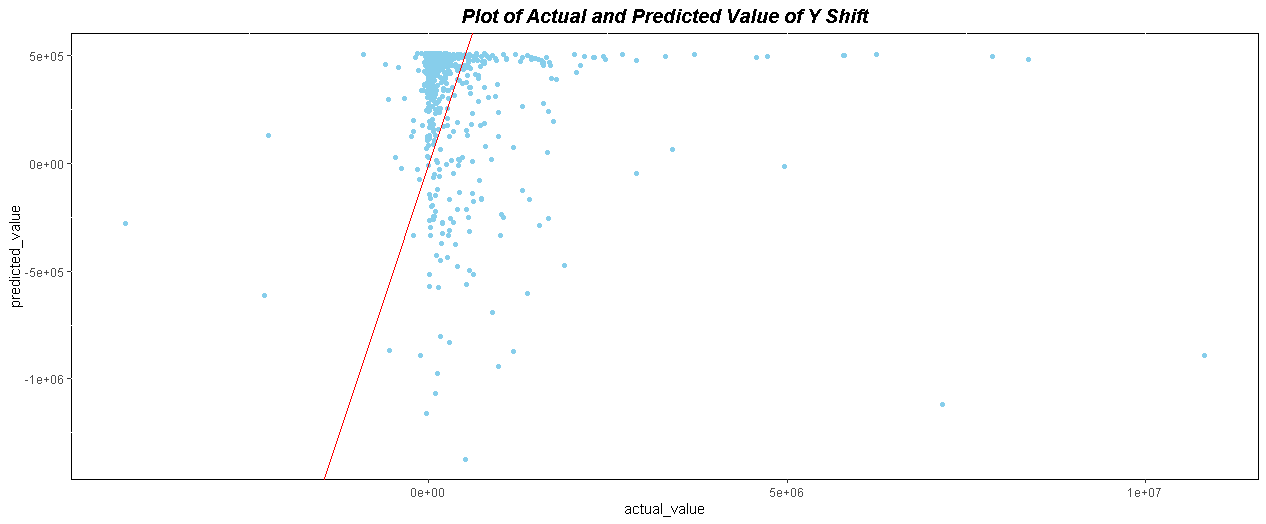
\includegraphics{../results/png/Actual_Predict_Y.png}

The second linear regression is performed between RBP2GOScore on x-axis
and x-shift on y-axis. The linear equation from the regression is
\(y = 0.069630x -0.368093\). The p value for the predictor variable y is
0.00285 and for x is 2e\textsuperscript{-16}. The p value of our model
is 2.2e\textsuperscript{-16} (\textbf{lm\_4}). The linear regression can
be seen in {[}7{]}. The QQ plot of the theoretical and sample residues
aligned with the QQ line except when the theoretical quantiles were
below -1.5 and above 1. The residuals were also plotted in a histogram
{[}8{]}.

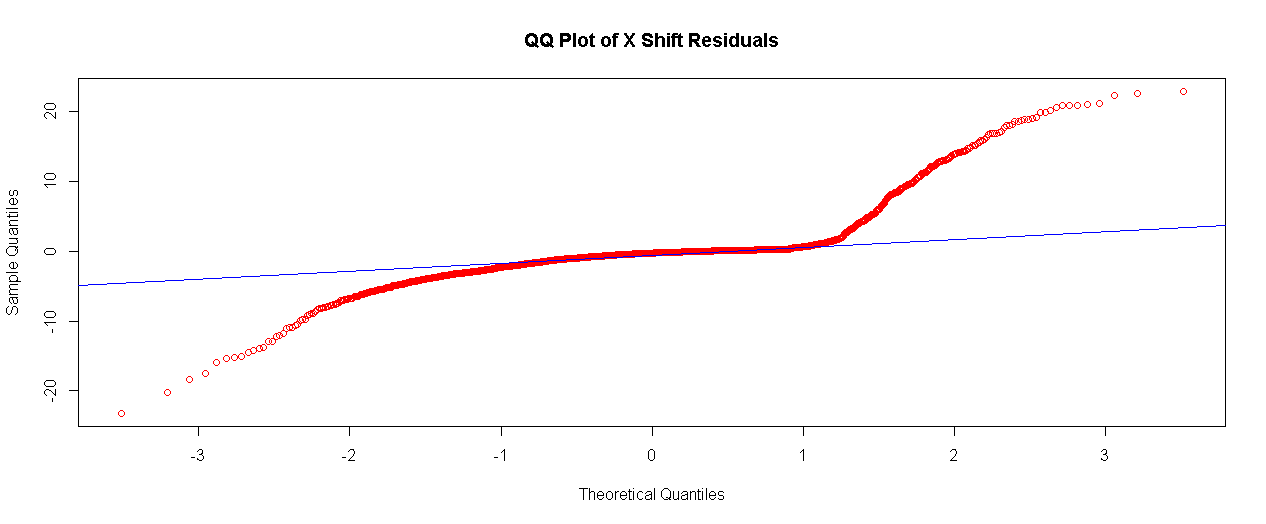
\includegraphics{../results/png/QQ_X.png}

The last plot was a plot with actual value in x axis, predicted value in
y axis and a linear line with intercept 0 and slope 1. The data points
were gathered mostly near the linear line when the actual value was
between -2 and 2 and the predicted value is around 0.5.

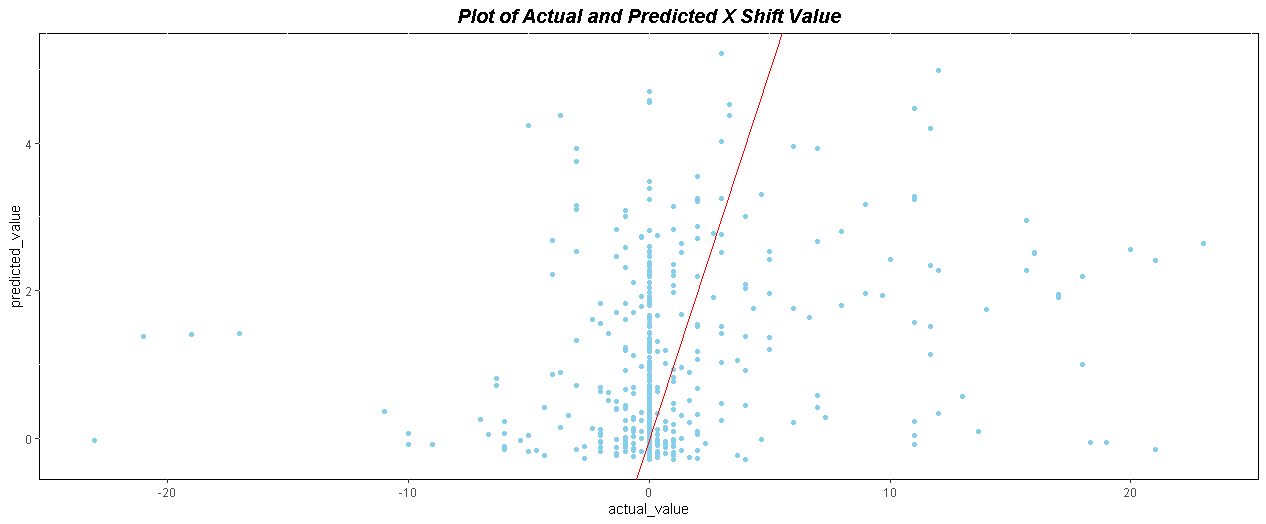
\includegraphics{../results/png/Actual_Predict_X.png}

\hypertarget{discussion}{%
\section{4. Discussion}\label{discussion}}

\hypertarget{normalization-fractionwise-normalization-and-anti-outlier-function}{%
\subsection{4.1 Normalization (Fractionwise Normalization and
Anti-Outlier
Function):}\label{normalization-fractionwise-normalization-and-anti-outlier-function}}

The normalization worked as expected. The total amount of protein per
replicate was equal for all Ctrl replicates and equal for all RNase
replicates, which made the replicates good and comparable. The
\textbf{df\_combi\_function} function did exactly what we wanted. The
outliers were reduced and did not have a significant effect on our data
after the normalization.

\hypertarget{peaks-identification-2}{%
\subsection{4.2 Peaks Identification:}\label{peaks-identification-2}}

The self-written \textbf{maximafunction} detected the global and local
maxima for different thresholds. To decide which threshold is the best
for the local maxima, we ran our \textbf{maxnum\_plot\_col} function,
which ploted a random protein with threshold in the x-axis and number of
maxima in y-axis. Having run the function several times, we decided to
use a threshold value of 40\% of the global maxima. Our chosen threshold
of 40\% was enough to get only significant maxima and reduce the effect
of noisy data.

\hypertarget{criteria-for-rna-dependency-2}{%
\subsection{4.3 Criteria for RNA
dependency}\label{criteria-for-rna-dependency-2}}

\hypertarget{criteria-for-rna-dependency-both-t-test-global-maximum-and-k-means-x--and-y-shift-for-global-maxima}{%
\subsubsection{4.3.1 Criteria for RNA dependency, both T-Test (global
maximum) and K-Means (X- and Y-shift for global
maxima):}\label{criteria-for-rna-dependency-both-t-test-global-maximum-and-k-means-x--and-y-shift-for-global-maxima}}

The H0 Hypothesis of the T-Test was there is no difference between Ctrl
and RNase group. And the H1 Hypothesis said that there was a difference
between these 2 groups. When the p-value of the test was below our alpha
significant value with additional Bonferroni correction to reduce
spurious positive results (0.05/number of t-test), then the respective
protein had a significant difference and consequently an RNA dependent
protein because we expect a migration of protein after RNAse treatment
in mass spectrometry.

The elbow method revealed that the optimal number of clusters was three.
It was determined through the kink from the elbow plot. The values of
our within cluster sum of squares of our 3 clusters were relatively low
and that means our clusters were pretty compact. There were 3 clusters
produced: the first cluster with most data has almost no Y-shift or even
negative shifts. The second cluster with 63 proteins, which have
positive X-shift and Y-Shift values. Lastly, the third cluster includes
only 4 proteins with very high negative Y-Shift values. We concluded
that the second cluster is RNA dependent protein because they have
positive Y-shift and X-Shift which proves that there are shifts of the
proteins. The other 2 clusters are RNA-independent proteins due to their
negative or almost zero values of Y-shift and the smallest cluster, it
seems to be outliers.

From the results of the T-test of global maxima and k means, We firstly
defined two criteria for RNA-dependency. The k-means clustering of the
Y-Shift and X-Shift and the T-Test significance for global maxima.
Although our defined two criteria could find RNA-dependent proteins with
a high true positive rate, the false negative rate was still too high.

\hypertarget{comparison-with-data-bank-with-two-criteria-1}{%
\subsubsection{4.3.2 Comparison with Data Bank with two
Criteria:}\label{comparison-with-data-bank-with-two-criteria-1}}

To find the proteins that fulfill the criteria for RNA dependency, we
compared the T-test results for a significant difference in the global
maxima for Ctrl and RNAse and the K means clustering (Y-shift and
X-shift detection) with the databank. The comparison with the table of
mammalian RNA-binding protein resources has shown that our applied
criteria find the RNA-dependent proteins with a very low false positive
rates, but very high false negative rates.

\hypertarget{comparison-with-data-bank-with-three-criteria-1}{%
\subsubsection{4.3.3 Comparison with Data Bank with three
Criteria:}\label{comparison-with-data-bank-with-three-criteria-1}}

To find more RNA dependent proteins, we included a 3rd criterion, T-test
results for local maxima to decrease the false negative and increase the
true positive rates. The H0 and H1 Hypothesis is identical to the T test
of global maxima with the corresponding Bonferroni correction. That
means, when the p-value was lower than the corrected alpha value, we
rejected the H0 Hypothesis and assumed the protein is RNA dependent and
otherwise when the p value was the same or bigger. As can be seen from
the table the false negative rate could be decreased but unfortunately,
our criteria were still not exact enough and the false negative rates
are still way too high. Nonetheless, our true positive and true negative
rates are higher.

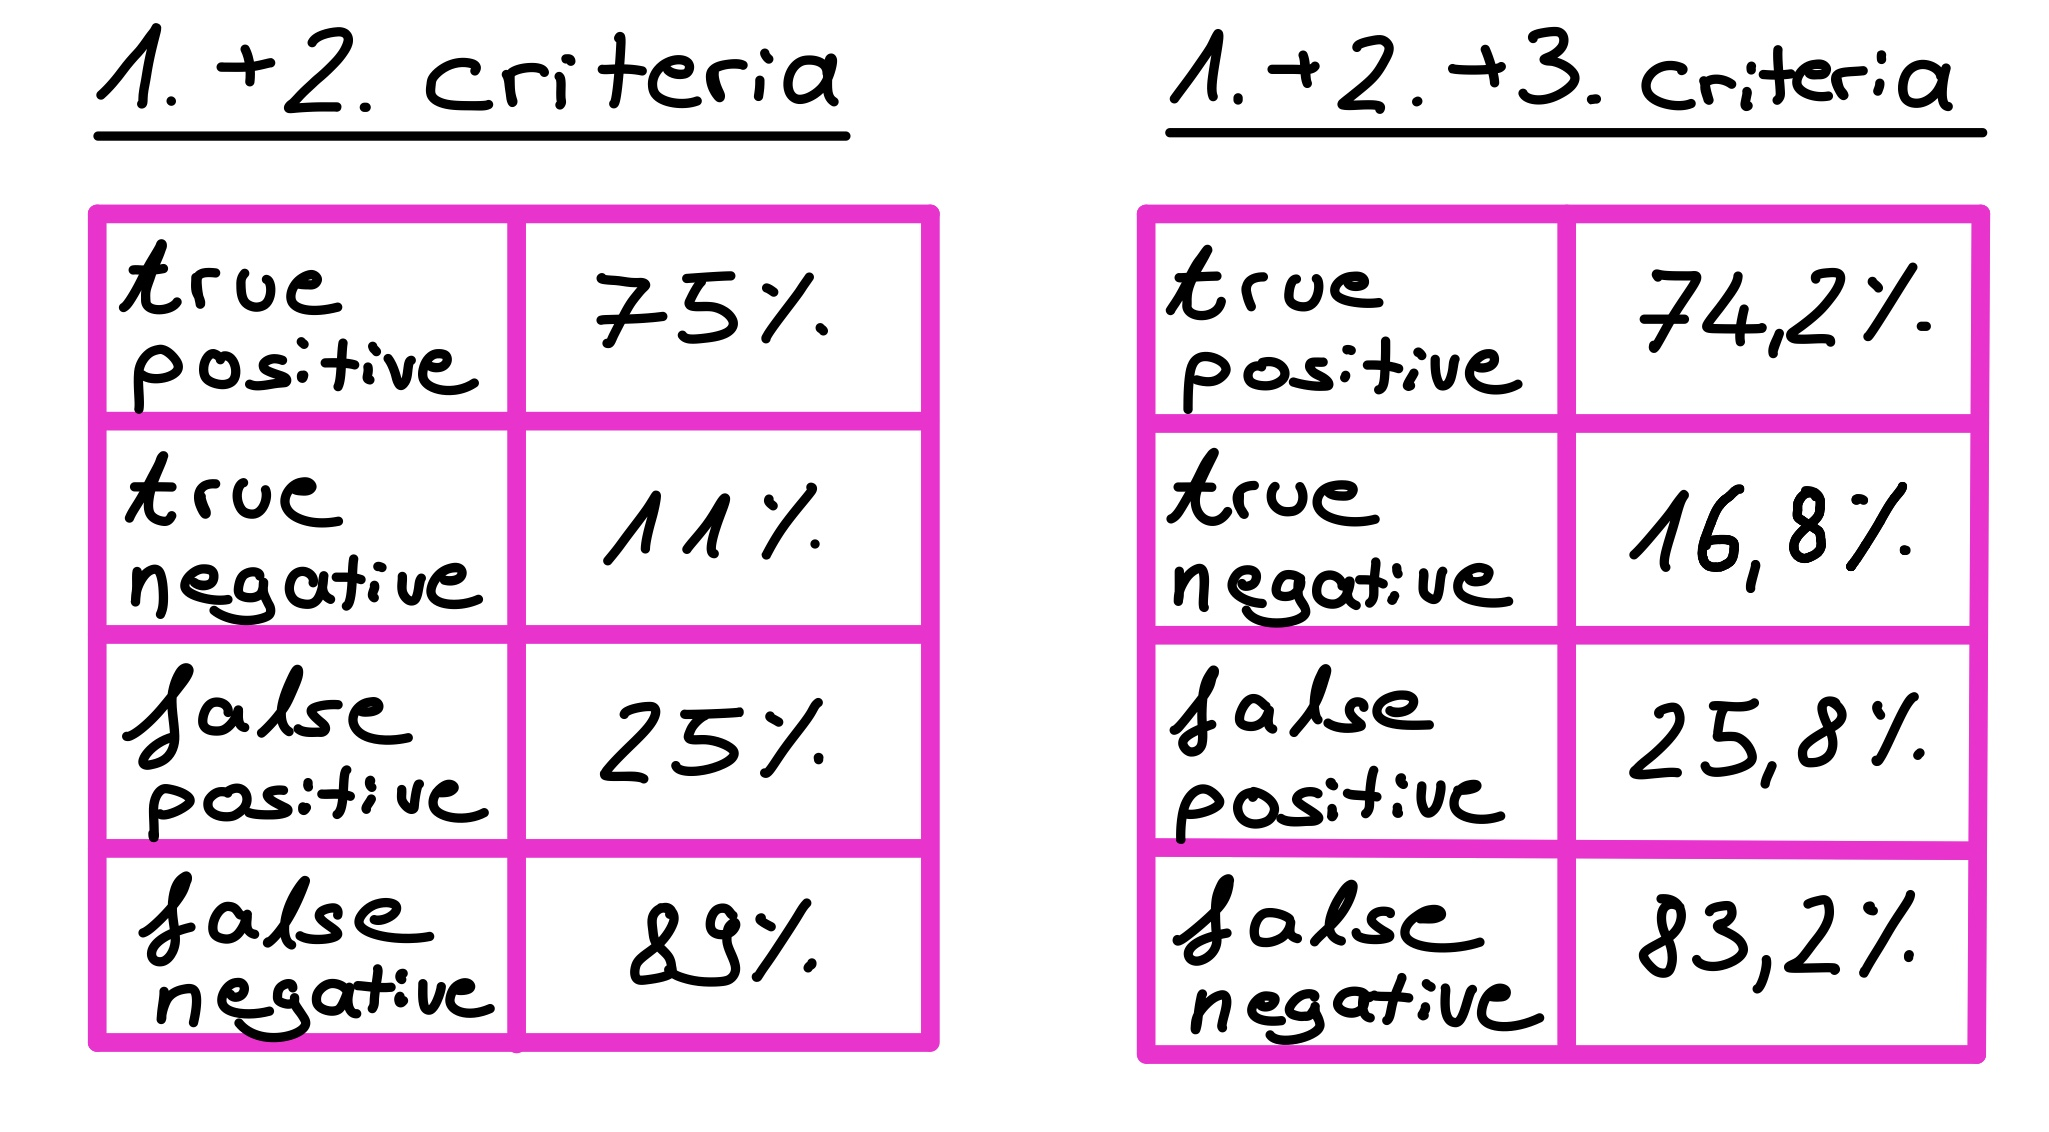
\includegraphics{../results/png/TrueFalseRates.png}

\hypertarget{linear-regression-between-y-shift-and-correlation}{%
\subsubsection{4.4.1 Linear Regression between Y-shift and
Correlation}\label{linear-regression-between-y-shift-and-correlation}}

The QQ plot showed us that the residuals were normally distributed with
heavy tails. The normal distribution of residues was centered at 0 and
showed that the model should fit the real values well. The plot of
predicted and actual values of Y shifts showed us, that the model didn't
work when the values were below 0. When the points were closer to the
line, it indicates that the predicted values were close to the actual
ones. Nevertheless, the model worked decently when the values are above
0. Sadly, the actual Y shift had a very high spread and made it hard to
find a perfect linear model to predict the Y shift.

\hypertarget{linear-regression-between-x-shift-and-rbp2go_score}{%
\subsubsection{4.4.2 Linear Regression between X-shift and
RBP2GO\_Score}\label{linear-regression-between-x-shift-and-rbp2go_score}}

The normal distribution of residues was proven through the QQ Plot
(heavy-tailed) with most of the residues centered at 0. The plot of
predicted and actual values of X shifts works fairly well when the X
shifts are very minimal (shift by one fraction). The linear model
unfortunately doesn't predict very well due to the variability of the X
shifts, especially when the shifts are higher.

\hypertarget{conclusion}{%
\section{5. Conclusion}\label{conclusion}}

One possible approach for better results could be using more replicates,
defining different criteria or maybe trying different data banks, since
we only compared our findings with one databank.

\hypertarget{references}{%
\section{6. References}\label{references}}

Caudron-Herger, M., Rusin, S.F., Adamo, M.E., Seiler, J., Schmid, V.K.,
Barreau, E., Kettenbach, A.N., and Diederichs, S. (2019). R-DeeP:
Proteome-wide and Quantitative Identification of RNA-Dependent Proteins
by Density Gradient Ultracentrifugation. Mol Cell 75, 184-199.e110.
10.1016/j.molcel.2019.04.018. Caudron-Herger, M., Wassmer, E., Nasa, I.,
Schultz, A.-S., Seiler, J., Kettenbach, A.N., and Diederichs, S. (2020).
Identification, quantification and bioinformatic analysis of
RNA-dependent proteins by RNase treatment and density gradient
ultracentrifugation using R-DeeP. Nature Protocols 15, 1338-1370.
10.1038/s41596-019-0261-4. Corley, M., Burns, M.C., and Yeo, G.W.
(2020). How RNA-Binding Proteins Interact with RNA: Molecules and
Mechanisms. Molecular Cell 78, 9-29. 10.1016/j.molcel.2020.03.011.
Gebauer, F., Schwarzl, T., Valcárcel, J., and Hentze, M.W. (2021).
RNA-binding proteins in human genetic disease. Nature Reviews Genetics
22, 185-198. 10.1038/s41576-020-00302-y. Liao, Y., Feng, J., Sun, W.,
Wu, C., Li, J., Jing, T., Liang, Y., Qian, Y., Liu, W., and Wang, H.
(2021). CIRP promotes the progression of non-small cell lung cancer
through activation of Wnt/β-catenin signaling via CTNNB1. Journal of
Experimental \& Clinical Cancer Research 40, 275.
10.1186/s13046-021-02080-9. Sternburg, E.L., and Karginov, F.V. (2020).
Global Approaches in Studying RNA-Binding Protein Interaction Networks.
Trends in Biochemical Sciences 45, 593-603. 10.1016/j.tibs.2020.03.005.

\hypertarget{attachment}{%
\section{7. Attachment}\label{attachment}}

\begin{figure}
\centering
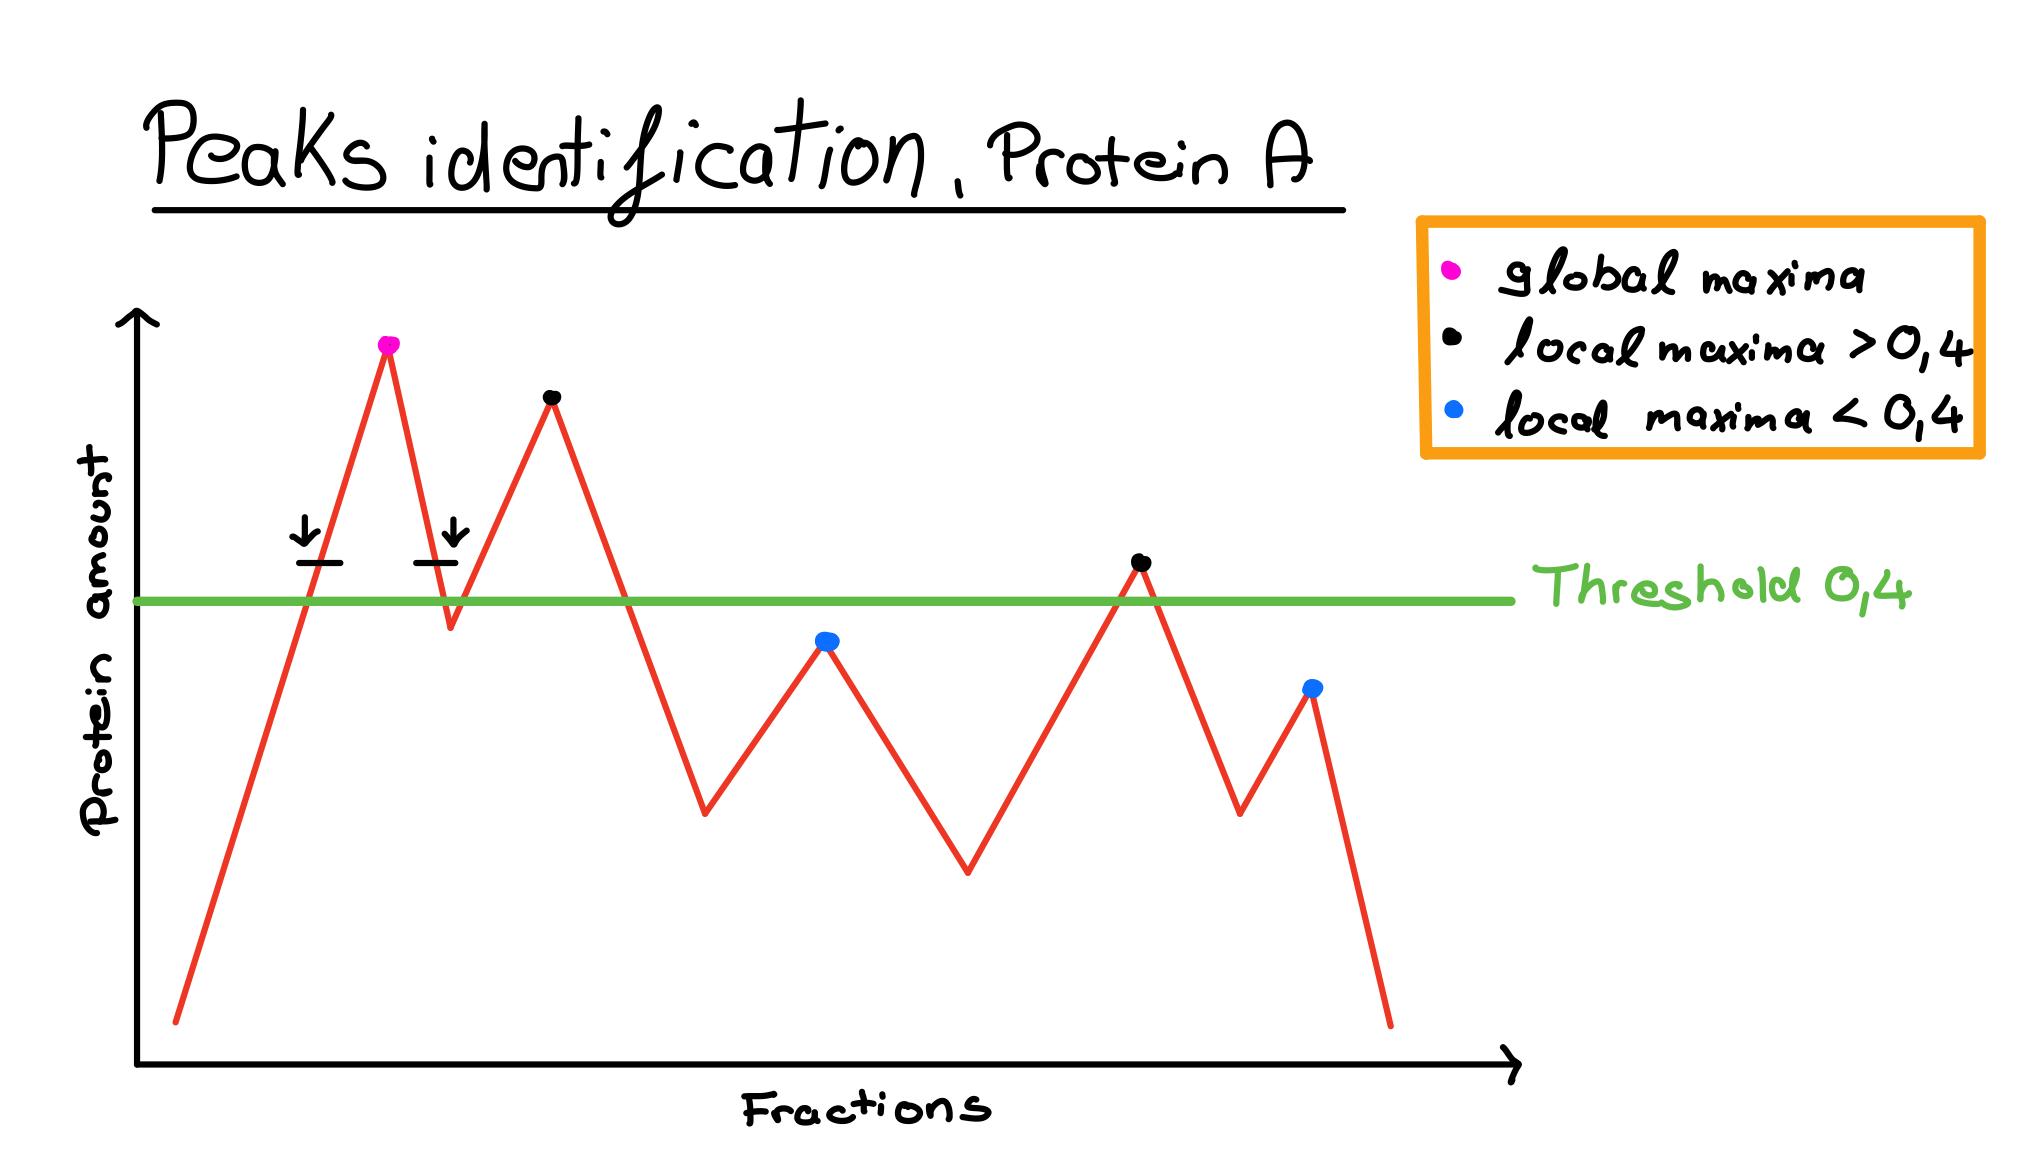
\includegraphics{../results/png/Peaks_identification_bild.png}
\caption{1}
\end{figure}

\begin{figure}
\centering
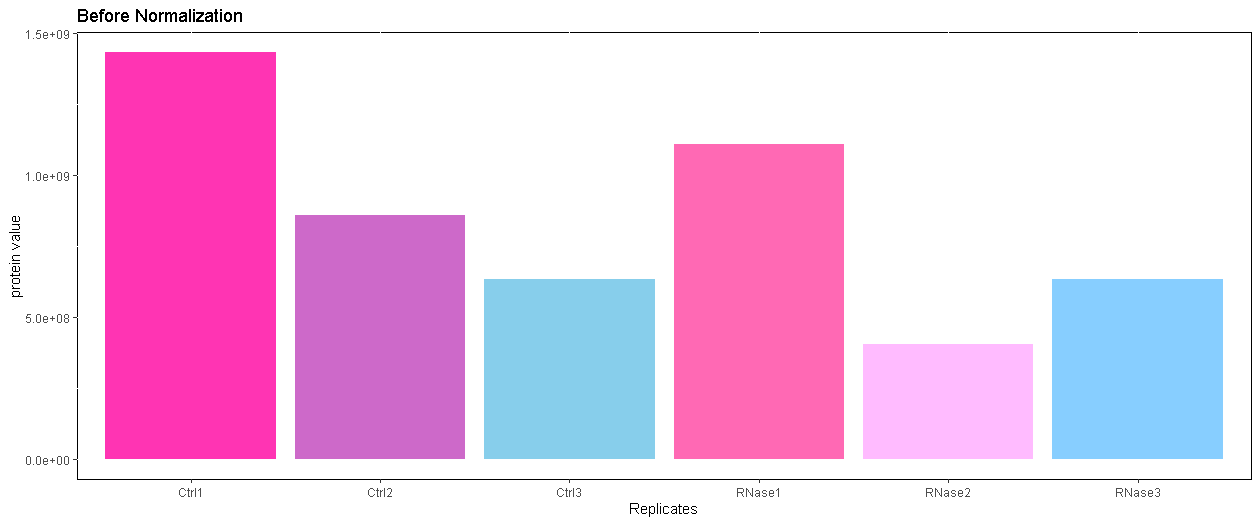
\includegraphics{../results/png/Before_Norm.png}
\caption{2}
\end{figure}

\begin{figure}
\centering
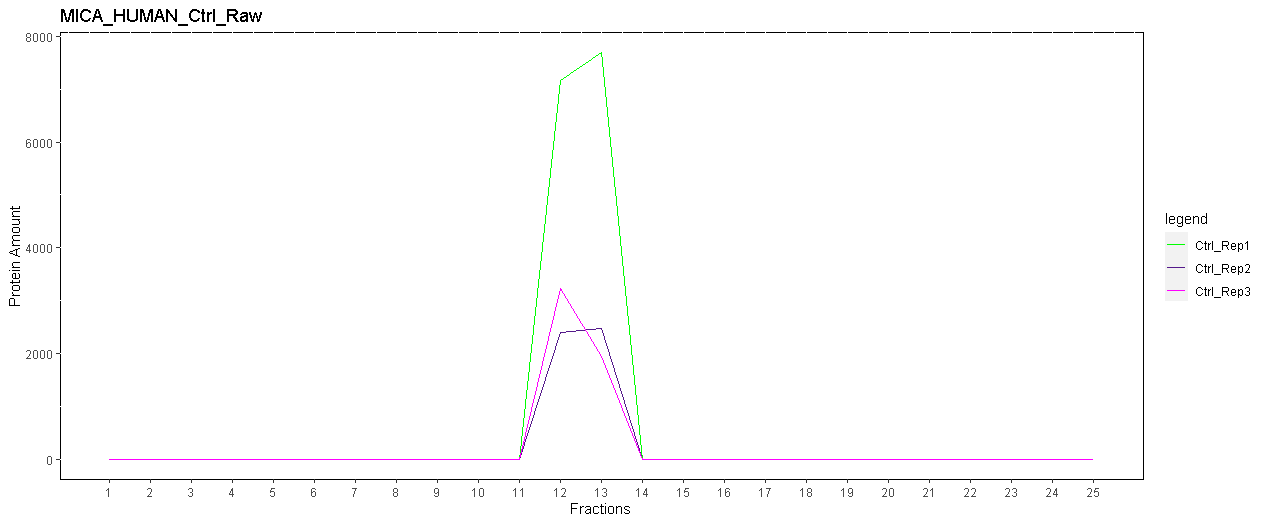
\includegraphics{../results/png/Ctrl_Raw.png}
\caption{3}
\end{figure}

\begin{figure}
\centering
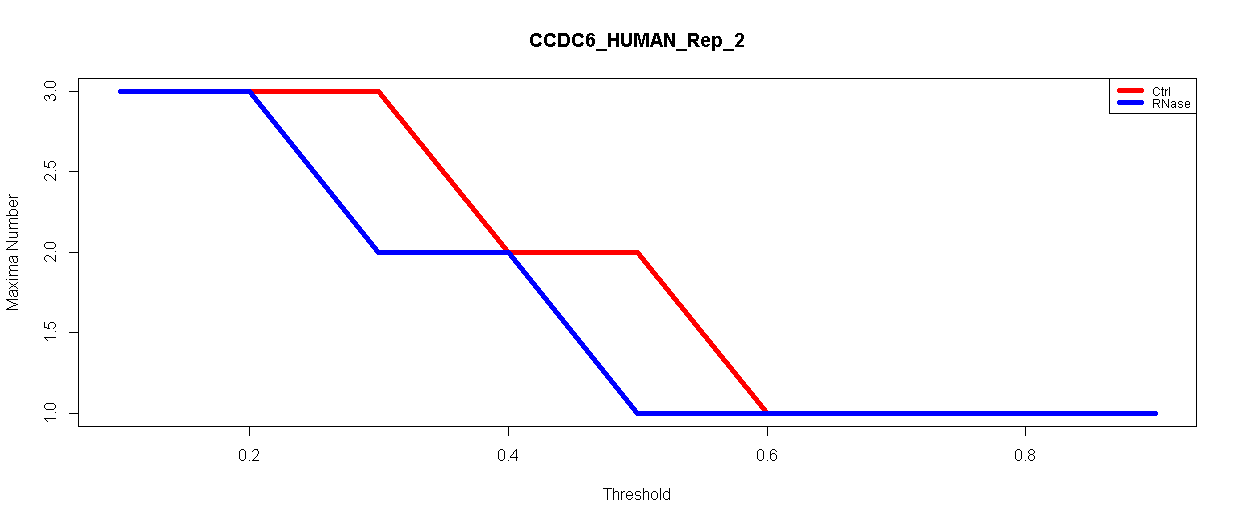
\includegraphics{../results/png/Maxnum_Plot.png}
\caption{4}
\end{figure}

\begin{figure}
\centering
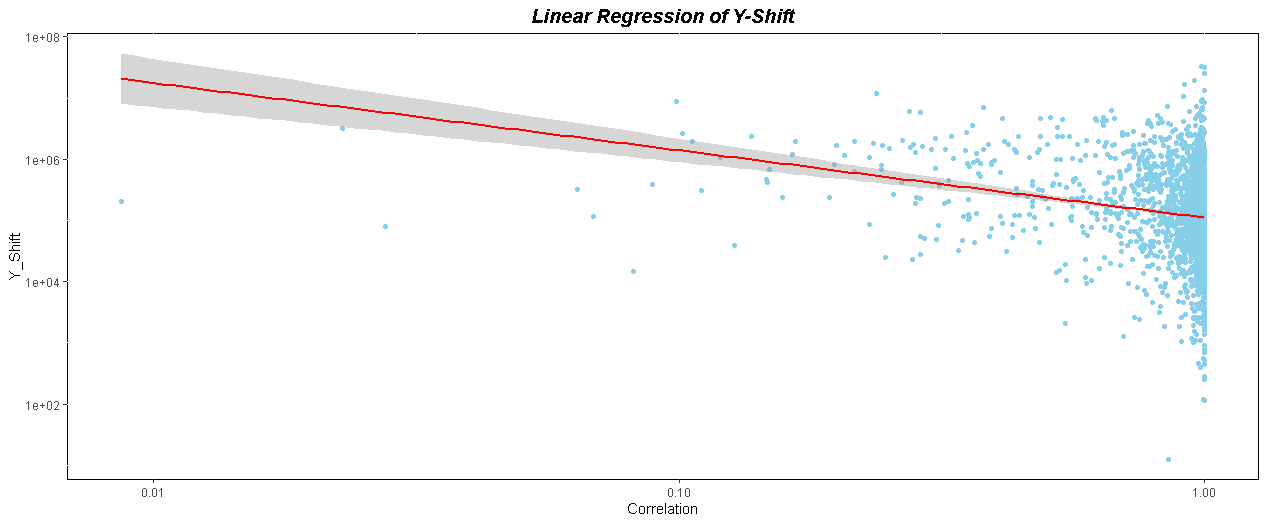
\includegraphics{../results/png/Regression_Y.png}
\caption{5}
\end{figure}

\begin{figure}
\centering
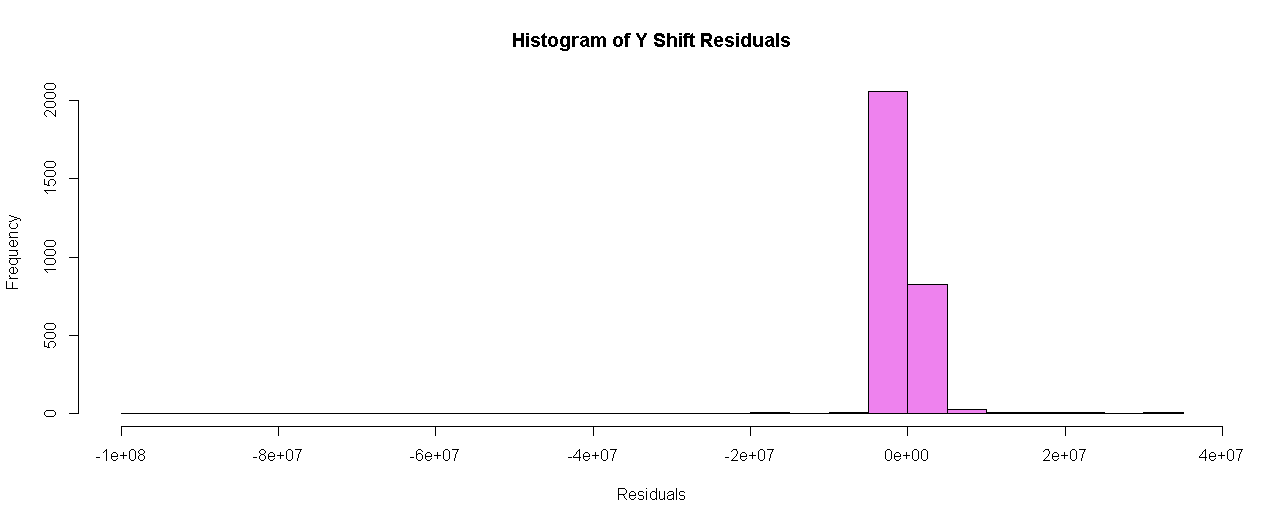
\includegraphics{../results/png/Hist_Y.png}
\caption{6}
\end{figure}

\begin{figure}
\centering
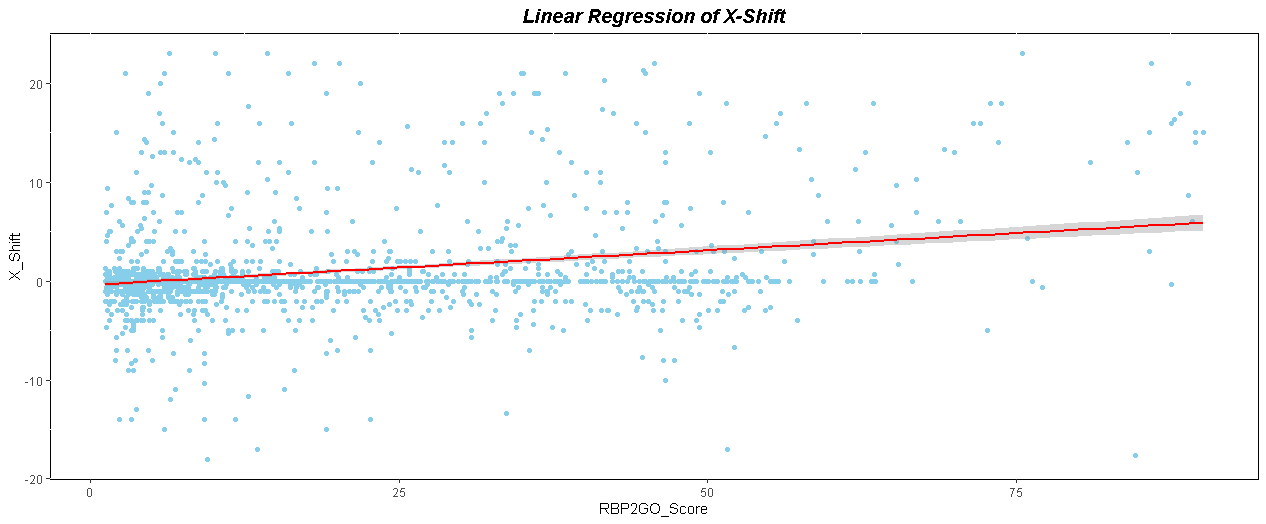
\includegraphics{../results/png/Regression_X.png}
\caption{7}
\end{figure}

\begin{figure}
\centering
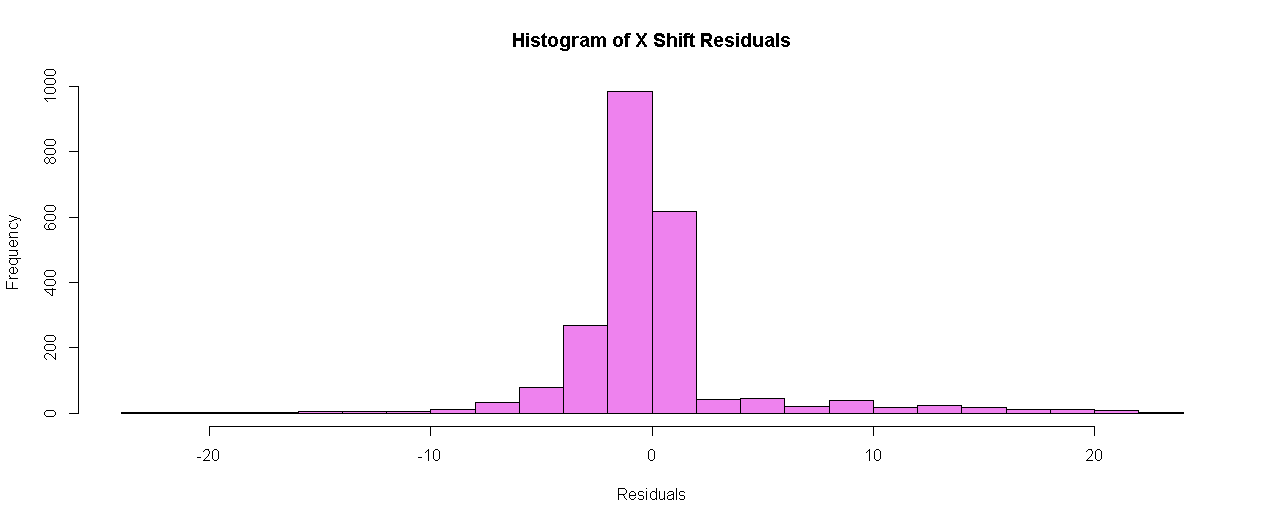
\includegraphics{../results/png/Hist_X.png}
\caption{8}
\end{figure}

\end{document}
